\section{Results and Evaluation}
\label{sec:brewrc-results} Parity matrices are considered sensitive
trade secrets. As in~\cite{patel2020bit}, the exact recovered parity
matrices are not disclosed. Instead, the extracted parity submatrices
are used to predict timing measurements for a fresh validation set of
1-word random unipolar walk test vectors, and the resulting timing
models are evaluated against both a naïve baseline and an independent
destructive reverse engineering result.

\subsection{Timing Model Construction}
Two systematic generator matrices $G_{4M}$ and $G_{8M}$ are constructed
by augmenting $I_{k_{4M}}$ and $I_{k_{8M}}$ with the extracted parity
matrices $P_{4M}$ and $P_{8M}$, respectively. $G_{4M}$ and $G_{8M}$ are
used to generate codeword transitions $(c_0, c_1)$ corresponding to
dataword transitions $(d_0, d_1)$ from the prior unipolar random walk
experiment. With full knowledge of the codeword transitions, the DHD for
each test vector can be computed at the codeword level. The median $t_w$
is computed for test vectors with identical $(w_{0\to1}, w_{1\to0})$
tuples. The timing model for each device is defined as a lookup table
keyed by DHD returning an expected median write time:
\begin{equation}
	\hat{t}_w(\delta) = \mathrm{Med}(t_w \mid \mathrm{DHD} = \delta).
\end{equation}
For comparison, a naïve timing model is generated using the same procedure but with dataword DHDs rather than codeword DHDs.

\subsection{Timing Model Performance}
\begin{figure}[t]
    \centering
    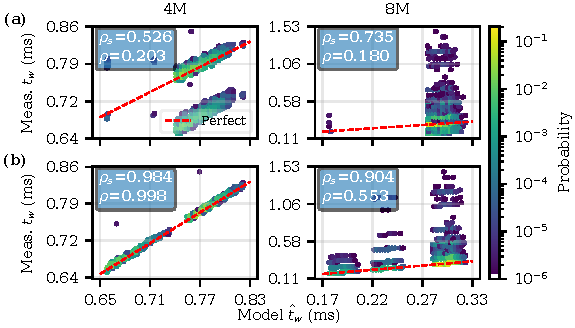
\includegraphics[width=\linewidth]{fig/images/pdf/model-comparison-codeword-vs-data.pdf}
    \vspace{-.75cm}
    \caption{Comparison of na\"ive dataword (a) and proposed codeword (b) timing models for 4M and 8M memories. Each point is colored according to the log probability that a measured $t_w$ occurs given a modeled $\hat{t}_w$.}
    % \vspace{-.2cm}
    \label{fig:timing-model}
\end{figure} A
fresh set of test vectors is generated for all 4M and 8M samples using
Algorithm~\ref{alg:ruw}. For the naïve model, $(d_0, d_1)$ transitions
are used directly to compute DHDs and lookup timing estimates. For the
proposed model, $G_{4M}$ and $G_{8M}$ are used to produce codewords and
the corresponding codeword DHDs are used for lookup. The test vectors
are applied to each chip and the raw $t_w$ is captured without
aggregation. Figure~\ref{fig:timing-model} compares the proposed
codeword-level timing model against the naïve dataword-level model. Both
Spearman and Pearson correlation coefficients are reported, as both are
relevant to side-channel analysis~\cite{batina2008comparative}. The
proposed model outperforms the naïve model on both devices. On the 4M,
the proposed model explains almost all $t_w$ variance. On the 8M, rare
long-tailed $t_w$ measurements limit the improvement, but a substantial
gain in both correlation metrics is still achieved. These results
demonstrate that the extracted parity submatrix yields accurate
codeword-level DHD computation, which substantially improves timing
leakage models.

\subsection{Validation Against Destructive Reverse Engineering}
Tay et al.~\cite{tay2023afm} used conductive-probe atomic force
microscopy to recover the logical-to-physical data mapping of the
MB85AS4MT, de-layering the device and probing it to determine the
physical destination of applied test vectors. They report 55 parity bits
for the device. Using $G_{4M}$, parity bits are generated for the same
set of test patterns. Since the correct physical mapping of the
extracted parity bits (i.e., the column order of $P$) and bit ordering
(MSB/LSB-first) cannot be known from timing alone, the minimum Hamming
distance between the 55 generated parity bits and the 55 reported parity
bits is computed across all possible $(5! \times 2)$ arrangements and
bit orders. One configuration produces a perfect match between generated
codewords and the parity bits reported by the authors; the next-best
configuration has a distance of 18 bits. This result confirms agreement
with destructive reverse engineering techniques and validates the
bit-exact recovery claim of BREW-RC.
